\documentclass[a4paper,10pt, notitlepage]{report}
\usepackage[utf8]{inputenc}
\usepackage{natbib}
\usepackage{amssymb}
\usepackage{amsmath}
\usepackage[shortlabels]{enumitem}
% \usepackage[portuguese]{babel}

\usepackage{hyperref}
\usepackage{url}
\usepackage{breqn}
\usepackage{multirow}
\usepackage{listings}

\newcommand{\ev}{\mathbb{E}}
\newcommand{\var}{\operatorname{Var}}
\newcommand{\cor}{\operatorname{Cor}}

\usepackage{xcolor}

\definecolor{codegreen}{rgb}{0,0.6,0}
\definecolor{codegray}{rgb}{0.5,0.5,0.5}
\definecolor{codepurple}{rgb}{0.58,0,0.82}
\definecolor{backcolour}{rgb}{0.95,0.95,0.92}

\lstdefinestyle{mystyle}{
    backgroundcolor=\color{backcolour},   
    commentstyle=\color{codegreen},
    keywordstyle=\color{magenta},
    numberstyle=\tiny\color{codegray},
    stringstyle=\color{codepurple},
    basicstyle=\ttfamily\footnotesize,
    breakatwhitespace=false,         
    breaklines=true,                 
    captionpos=b,                    
    keepspaces=true,                 
    numbers=left,                    
    numbersep=3pt,                  
    showspaces=false,                
    showstringspaces=false,
    showtabs=false,                  
    tabsize=1
}
\lstset{style=mystyle}


% Title Page
\title{Assignment II: Advanced simulation techniques.}
\author{Computational Statistics \\ Instructor: Luiz Max de Carvalho \\ Student: Lucas Machado Moschen}

\begin{document}
\maketitle

\textbf{Hand-in date: 08/12/2021.}

\section*{Background}

We have by now hopefully acquired a solid theoretical understanding of simulation techniques, including Markov chain Monte Carlo (MCMC).
In this assignment, we shall re-visit some of the main techniques in the field of Simulation.
The goal is to broaden your knowledge of the field by implementing one of the many variations on the general theme of simulation algorithms.

Each method/paper brings its own advantages and pitfalls, and each explores a slightly different aspect of Computational Statistics.
You should pick~\textbf{one} of the listed papers and answer the associated questions.

In what follows, ESS stands for effective sample size, and is similar to
$n_{\text{eff}}$ we have encountered before: it measures the number of
effectively uncorrelated samples in a given collection of random variates.

\section*{Paper Bootstrap~\citep{Efron1986}}

In orthodox (frequentist) Statistics, it is common to want to ascertain long run (frequency) properties of estimators, including coverage of confidence intervals and standard errors.
Unfortunately, for the models of interest in actual practice, constructing confidence intervals directly (exactly) is difficult.
The bootstrap method is a re-sampling technique that allows for a simple yet theoretically grounded way of constructing confidence intervals and assessing standard errors in quite complex situations.

For this assigment, you are encouraged to consult the seminal 1986 review by stellar statisticians Bradley Efron and Robert Tibshirani~\citep{Efron1986}.

\textit{Hint:} Brush off on your Normal theory before delving in.
The book by \cite{Schervish2012} -- specially Chapter 5 -- is a great resource.

\begin{enumerate}
 \item Define and explain the bootstrap technique;
 \item Define and explain the jackknife technique;
 \item Implementation:
\begin{enumerate}[(a)]
   \item Reproduce the results in Table I of~\cite{Efron1986};
   \item Show what happens if one increases/decreases the value of $B$;
 \end{enumerate} 
 \item Why is it important to draw exactly $n$ samples in each bootstrap iteration? Can this be relaxed?
 \item (bonus) Propose an alternative bootstrap method to the one proposed in the paper and discuss the situations where the new method is expected to perform better.
\end{enumerate}

\section*{Bootstrap}

{\em Bootstrap} is a technique for measuring the accuracy of an estimator through
approximations for standard errors and confidence intervals. The
frequentist inference approach has several usages for bootstrap, but it can be
interpreted in the Bayesian framework \cite[]{rubin1981bayesian}. From
samples of an experiment, the general idea is to generate new data points, and perform the
estimation process for each one. This procedure creates an {\em empirical
distribution} for the considered estimator, such as the {\em maximum likelihood
estimator} (MLE).

The construction from \cite{Efron1986} supposes that $\boldsymbol{x} = (x_1, x_2,
\dots, x_n)$ is an observation of the independent and identically distributed
random variables 
$$
\boldsymbol{X} = (X_1, X_2, \dots, X_n), X_i \overset{iid}{\sim} F, 
$$
where $F$ is an unknown probability distribution. This assumption can be
relaxed for dependent data using block bootstrap strategies
\cite[]{lahiri1999theoretical}. Let $R(\boldsymbol{X}, F)$ be a random 
variable of interest, such as the statistic $\hat{\theta}(\boldsymbol{X})$. 
From sample $\boldsymbol{x}$, we build the empirical distribution
$\hat{F}$, that is, if $X \sim \hat{F}$, we have $\Pr(X = x_i) = 1/n$.

The bootstrap technique offers a 
Monte Carlo estimator for some characteristic of the distribution of $R$, such
as its mean $\ev_{\hat{F}}[R]$. A common example of interest is the 
standard error 
$$\sigma_F = \left(\var_F(\hat{\theta}(\boldsymbol{X}))\right)^{1/2}$$
of a statistic $\hat{\theta}(\boldsymbol{X})$ 
which can be approximated\footnote{This is proved under some regularity conditions.} by 
$$
\hat{\sigma}_{\hat{F}} = \left(\var(\hat{\theta}_
{\hat{F}}(\boldsymbol{x}))\right)^{1/2}
$$
the standard deviation at $F = \hat{F}$. 

We know how to draw from $\hat{F}$: sampling with replacement from $\{x_1, \dots, x_n\}
$. With that, we obtain $B$ {\em bootstrap samples} $\boldsymbol{x}^{(1)},
\dots, \boldsymbol{x}^{(B)}$ with fixed size $n$. As usual for Monte Carlo estimators, for each bootstrap sample
$\boldsymbol{x}^{(i)}$, we evaluate $R^{(i)} = R(\boldsymbol{x}^{(i)},
\hat{F})$, obtaining samples $\{R^{(1)}, \dots, R^{(B)}\}$. Then, we calculate
the quantity of interest, such as 
$$
\frac{1}{B}\sum_{i=1}^B R^{(i)} \overset{P}{\to} \ev_{\hat{F}}[R], 
$$
where $P$ indicates convergence in probability as a result of the Strong Law
of Large Numbers (SLLN). 

For the standard error approximation of $\hat{\sigma}_{\hat{F}}$ we use 
$$
\hat{\sigma}_B = \left(\frac{1}{B-1}\sum_{i=1}^B (\hat{\theta}(\boldsymbol{x}^{(i)}) - \hat{\theta}^B)^2\right)^{1/2},
$$
where $\hat{\theta}(\boldsymbol{x}^{(i)})$ is the statistic of interest evaluated in
$\boldsymbol{x}^{(i)}$ and 
$$\hat{\theta}^B = B^{-1}\sum_{i=1}^B
\hat{\theta}(\boldsymbol{x}^{(i)}).$$ 
In the same sense, by the SLLN, 
$$
\hat{\sigma}_B \overset{P}{\to} \hat{\sigma}_{\hat{F}}.
$$

Notice that $R(\boldsymbol{X}, F)$ depends on $n$ through $\boldsymbol{X}$.
For instance, if $\hat{\theta}(\boldsymbol{X})$ is a strongly consistent estimator for
$\theta$, it gets close to $\theta$ with probability one. In that sense the
standard error of the estimator vanishes when $n$ tends to infinity. This
shows that the distribution of $\hat{\theta}(\boldsymbol{X})$ changes with
$n$ with its limit being a punctual mass in $\theta$. Since the distribution
changes with $n$, we cannot get bootstrap samples with different sizes and use
Monte Carlo estimator as we are current doing. In summary, it is important to
draw bootstrap samples with size $n$ to get samples from the same
distribution $\hat{F}$ and, hence, $\hat{\theta}(\boldsymbol{x})$.
\cite{bickel1981some} presents a situation where the bootstrap sample size $m$
is different from $n$ for approximating the finite mean $\mu$ of $F$. 

We presented above the non-parametric form of bootstrap. If we believe that
$F$ belongs to a family, we can estimate it through its parametric MLE. For
instance, if we believe that $F$ comes from the normal distribution, its MLE
is the normal distribution with mean $\bar{x}$ and variance $s^2$, where
$\bar{x}$ is the sample mean and $s^2$ is the unbiased sample variance. 

\section*{Bayesian Bootstrap}

The {\em Bayesian bootstrap} (BB) generates a posterior distribution for
each $x_i$ such that not observed values have zero posterior probability. The 
posterior probability for each $x_i$ is centered at $1/n$ with some
variability. The ideia is to generate $u_1, \dots, u_{n-1} \overset{iid}{\sim}
\operatorname{Unif}[0,1]$ and get the order statistics $u_{(1)}, \dots,
u_{(n-1)}$. At last, we define $g_i = u_{(i)} - u_{(i-1)}$, where
$i=1,\dots,n$ and $u_{(0)} = 0, u_{(n)} = 1$. Then we attach probability $g_i$
for $x_i$, which obtains a replication for the data. 

For instance, suppose we are interested in the mean of the random variable
$X$. Then, the posterior distribution of the posterior mean is $\sum_{i=1}^n
g_i^{(l)} x_i$, such that $g_i^{(l)}$ is the $i$-th probability of the $l$-th
Bayesian replication.

The distribution generated by Bayesian bootstrap is similar to the regular
one, but \cite{rubin1981bayesian} argues that BB has an advantage regarding
the interpretation since it generates probability statements about the
parameters, rather than frequency of statistics.

We implemented this bootstrap, but the results were different from what we
expected, since the standard error was less than the other two approaches.
More work should be done to correct implementation bugs.

\section*{Jackknife technique}

{\em Jackknife} is a re-sampling method to estimate bias and variance of estimators,
which pre-dates bootstrap. The basic idea is to leave out one observation per
time and calculate the estimated quantity for this reduced sample. The average of
these calculations is the jackknife estimate. We denote $\boldsymbol{x}_{(i)}$
the sample except the observation $i$, i.e., 
$$
\boldsymbol{x}_{(i)} = (x_1, x_2, \dots, x_{i-1}, x_{i+1}, \dots, x_n).
$$
This is the {\em jackknife} sample $i$. An estimate for $\sigma_F$ is 
$$
\hat{\sigma}_J = \sqrt{\frac{n-1}{n}\sum_{i=1}^n (\hat{\theta}(\boldsymbol{x}_{(i)}) - \hat{\theta}^J)^2}, 
$$
where $\hat{\theta}^J = \sum_{i=1}^n \hat{\theta}(\boldsymbol{x}_i)/n$.

\section*{Results in Table I}

The experiment is as follows: set $n=15$ and the statistic of interest
$\hat{\theta}$ is the 25\% trimmed mean. The $100\alpha$ trimmed mean discard
the $\alpha$ highest and $\alpha$ lowest in the sample and calculate the mean
with the other $n(1 - 2\alpha)$ data points. Let $x_{(1)} \le \dots \le
x_{(n)}$ be the order statistic of $\boldsymbol{x}$. Let $g$ be the integer
and $r$ the fraction part of $n\alpha$. The trimmed mean is 
$$
\bar{x}_{\alpha} = \frac{1}{n(1-2\alpha)} \left((1-r)(x_{(g+1)} + x_{(n-g)}) + \sum_{i=g+2}^{n-g-1} x_{(i)}\right).
$$
In our case, $15\cdot 0.25 = 3.75$, then 
$$
\bar{x}_{.25} = \frac{1}{7.5}\left(0.25(x_{(4)} + x_{(12)}) + \sum_{i=5}^{11} x_{(i)}\right).
$$
Since we could not calculate the standard error of $\bar{x}_{\alpha}$
analytically, we propose a Monte Calor estimator. We have that, 
\begin{align*}
  \var(\bar{x}_{\alpha}) &= \frac{1}{n^2(1-2\alpha)^2}\left(\sum_{i,j=g+2}^{n-g-1} \cor(X_{(i)}, X_{(j)}) \right. \\
  &+ \left. 2(1-r)\sum_{i=g+2}^{n-g-1} \cor(X_{(g+1)}, X_{(i)}) + \cor(X_{(n-g)}, X_{(i)})\right. \\ 
  &+ \left. (1-r)^2\left(\cor(X_{(g+1)}, X_{(g+1)}) + 2\cor(X_{(g+1)}, X_{(n-g)}) \right. \right. \\
  &\hspace{2cm} + \left. \left. \cor(X_{(n-g)}, X_{(n-g)})\right)\right),
\end{align*}
and $\cor(X_{(i)}, X_{(j)})$ can be calculated sampling $X_{(i)}$ and
$X_{(j)}$ from distribution $F$. We consider two different probability
distributions for $F$, (i) standard normal, and (ii) exponential with
parameter $\lambda = 1$. Moreover, in order to provide a standard deviation for $\hat{\sigma}_B$ we
analyse its variability for different data points $\boldsymbol{x}$ drawn from
distribution $F$. We also calculate the coefficient of variation.
\autoref{tab:table1} summarizes the results. The Jackknife is a little closer
than bootstrap, but has a larger standard deviation.  Both estimates are good
for the standard deviation these simple situations. We also note that $B=200$
already provide good estimates and $B=10000$ is 50 times more expensive, but
reduced the standard deviation very little.

\begin{table}[htb]
  \centering
  \begin{tabular}{ccccccc}
  \hline
  \multirow{2}{*}{Method} & \multicolumn{3}{c}{F standard normal} & \multicolumn{3}{c}{F exponential $\lambda = 1$} \\ \cline{2-7} 
   & Average & SD & CV & Average & SD & CV \\ \hline
  Bootstrap ($200$) & 0.285 & 0.071 & 0.249 & 0.239 & 0.083 & 0.347 \\
  Bootstrap ($10000$) & 0.285 & 0.07 & 0.246 & 0.241 & 0.082 & 0.34 \\
  Jackknife & 0.277 & 0.081 & 0.292 & 0.243 & 0.093 & 0.383 \\
  True value ($10^6$) & 0.28 &  &  & 0.236 &  &  \\ \hline
  \end{tabular}
  \caption{\label{tab:table1}Sampling experiment comparing bootstrap with
  $B=200$ and $B=10000$ samples and Jackknife estimates of standard error for
  the 25\% trimmed mean with $n=15$ for the standard normal and exponential
  distribution. We denote CV for the coefficient of variation and SD the
  standard deviation. The true value is calculated performing the estimates
  for $10^6$ different samples from $F$ and calculating the corresponding
  Monte Carlo estimate.}
\end{table}

\autoref{fig:figure1} presents the standard deviation calculation for different values of
$B$. It would be nice to perform this curve more times to observe the
variability with respect to different values of $B$, but this would be too
computationally expensive.  Notice that bootstrap generates biased estimates as $B$ grows.

\begin{figure}[htb]
  \centering
  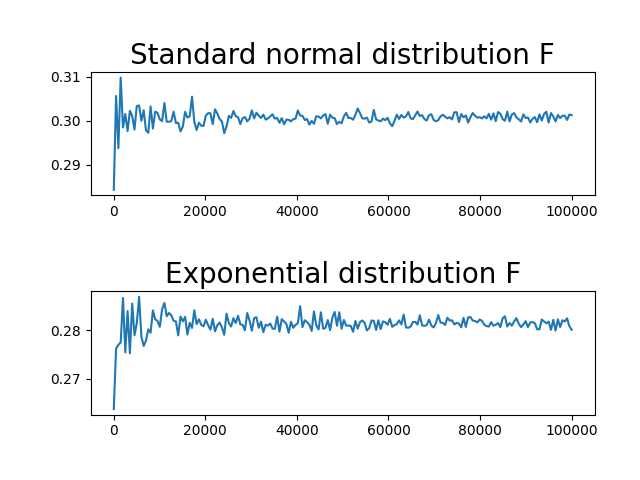
\includegraphics[width=0.6\textwidth]{different_values_B.png}
  \caption{\label{fig:figure1}Convergence of the Bootstrap standard error
  estimator for the 25\% trimmed mean for different values of $B$.}
\end{figure}

Finally, \autoref{fig:figure2} shows four situations: we consider two
datasets, one generated drawn by the standard normal distribution, while the
other by the standard t-Student with 5 degrees of freedom. The parametric
approach is considered using the standard normal for both cases. This graphic
suggests not much difference, but supposing a normal distribution instead of
t-Student led to a more variable histogram, including values next to 1.

\begin{figure}[htb]
  \centering
  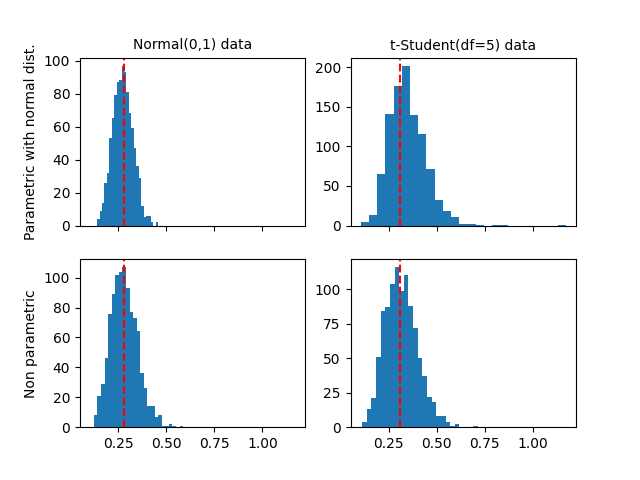
\includegraphics[width=0.6\textwidth]{parametric_bootstrap.png}
  \caption{\label{fig:figure2}Histogram of the values of bootstrap standard errors
  with different datasets and different bootstrap approaches.}
\end{figure}

We finally present the difference between the Bayesian and regular bootstraps
to present the implementation code we had. \autoref{fig:figure3} shows that
although the the posterior mean of the trimmed mean distribution is close to
the bootstrap mean, the variability is very difference, in a way that the
Bayesian is underestimating the real accuracy of this statistic.

\begin{figure}[htb]
  \centering
  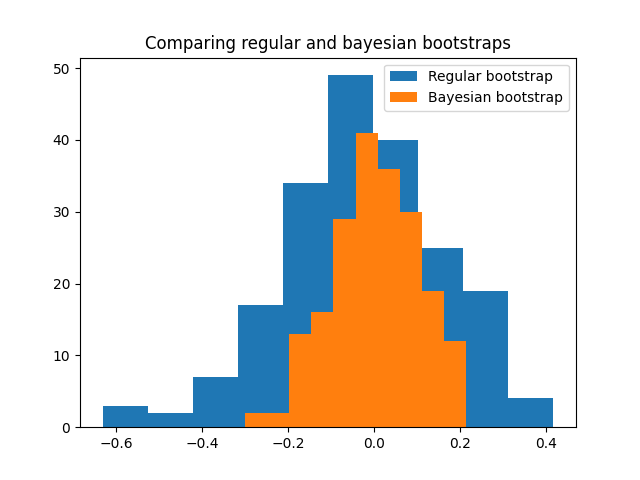
\includegraphics[width=0.6\textwidth]{baysian-vs-bootstrap.png}
  \caption{\label{fig:figure3}Histograms comparing the posterior distribution
  and the regular bootstrap distribution of the trimmed mean in the standard
  normal case.}
\end{figure}

\section*{Python code of the implementation}

\lstinputlisting[language=Python, 
                 firstline=7, 
                 lastline=151]{implementation.py}

\def\mynumber{0}
\if\mynumber1

\section*{Paper summary}

\begin{enumerate}
  \item Bootstrap is a general methodology for answering how accurate an
  estimator is. 
  \item Suppose $X_1, \dots, X_n \sim F.$
  \item Let the sample mean $\bar{x}$ be an estimate for $\theta = \ev[X_1]$.
  \item The standard error is a measure of $\bar{x}$ accuracy. We usually use its
  estimator form.
  \item Let $\hat{F}$ be the empirical probability distribution that poses mas
 $1/n$ for each observed data point $x_1$.
 \item The bootstrap estimator is the standard deviation of $\hat{F}$.
 \item Assumes the samples are independent and identically distributed
 \item Let $\hat{\theta}(x)$ a statistic of interest.
 \item We sample $n$ independent draws from $\hat{F}$, which is equivalently
 to resample with replacement. We call this new sample of bootstrap sample.
 Calculate the the statistic of interest for each bootstrap sample. 
 \item It's easy see that $B \to \infty$ implies convergence. 
 \item The MC estimator will not converge to the true standard deviation if
 the bootstrap sample size differs from $n$. Bickel and Freedman (1981) showed
 how to relax this. 
 \item parametric bootstrap
 \item Fisher information estimator for standard error are essentially
 bootstrap estimates in parametric framework.
 \item Example of table 1: 25\% trimmed mean. 
 \item Discussion about $B$ size.
 \item The jackknife approximation is the linear function of the probabilities
which matches the estimator at the $n$ points. 
  \item There is a relation between these estimators
\end{enumerate}

\fi

\bibliographystyle{apalike}
\bibliography{stat_comp}

\end{document}          
